\section{Reading potentiometer from Scilab}
\subsection{Reading the potentiometer}
In this section, we will use a Scilab script to read the potentiometer
values.  Based on the acquired potentiometer values, we will change
the state of the RGB LED. The Shield has to be attached to the \arduino\ board
before doing these experiments and the \arduino\ needs to be connected to the computer 
with a USB cable, as shown in \figref{arduino}.
The reader should go through the instructions given in
\secref{sec:sci-start} before getting started. 

As explained earlier, the potentiometer values range from 0 to 1023. We will divide this entire range into 3
bands, 0-319, 320-900, and 901-1023. For each read value, we use an
{\tt if elseif} statement and correspondingly turn on either the Red,
Green or Blue LED. The code for this experiment is given in
\sciref{sci:pot-100}. We start the experiment by opening the serial
port for communication between \scilab\ and the \arduino\ board. Then,
we read the analog input at pin 2 using,
\lstinputlisting[firstline=4,lastline=4]
                {\LocPotscicode/pot-threshold.sce} where the first
                argument is for
%\redcolor {the kit number } 
the kit number and the second argument corresponds to the analog pin to be read.  Next, we compare the read values with the set threshold, 
and then turn on and off the corresponding LED. For example, 
\lstinputlisting[firstline=6,lastline=9]
{\LocPotscicode/pot-threshold.sce} where {\tt cmd\_digital\_out} 
is used to set the pin 11 high (1) or low (0). 
We used {\tt sleep(1000)} to retain the LED in the on state for 
1000 milliseconds.  
A similar check is done for the other two bands. 
While running this experiment, 
the readers must rotate the knob of the potentiometer and observe 
the change in the color of the RGB LED. 

\subsection{Scilab Code}
\label{sec:pot-scilab-code}
\addtocontents{cod}{\protect\addvspace{\codclr}}
\begin{scicode}
  \ccaption{Turning on LEDs depending on the potentiometer
    threshold}{Turning on LEDs depending on the potentiometer
    threshold.  Available at
  \LocPotscibrief{pot-threshold.sce}.}
\label{sci:pot-100}
\lstinputlisting{\LocPotscicode/pot-threshold.sce}
\end{scicode}

\section{Reading potentiometer from Xcos}
In this section, we discuss how to read the potentiometer values using
Xcos blocks. When the file required for this experiment is invoked, one
gets the GUI as in \figref{fig:pot-threshold}.  In the caption of this
figure, one can see where to locate the file.  The reader should go
through the instructions given in \secref{sec:xcos-start} before
getting started.

In this experiment, the block {\tt Analog Read Pin 2} performs the read 
operation from pin 2. The threshold is set using the block, {\tt Dynamic}. 
Depending on the condition met, a $1$ or $0$ is given to pin 9, 10 or 11.

\begin{figure}
  \centering
  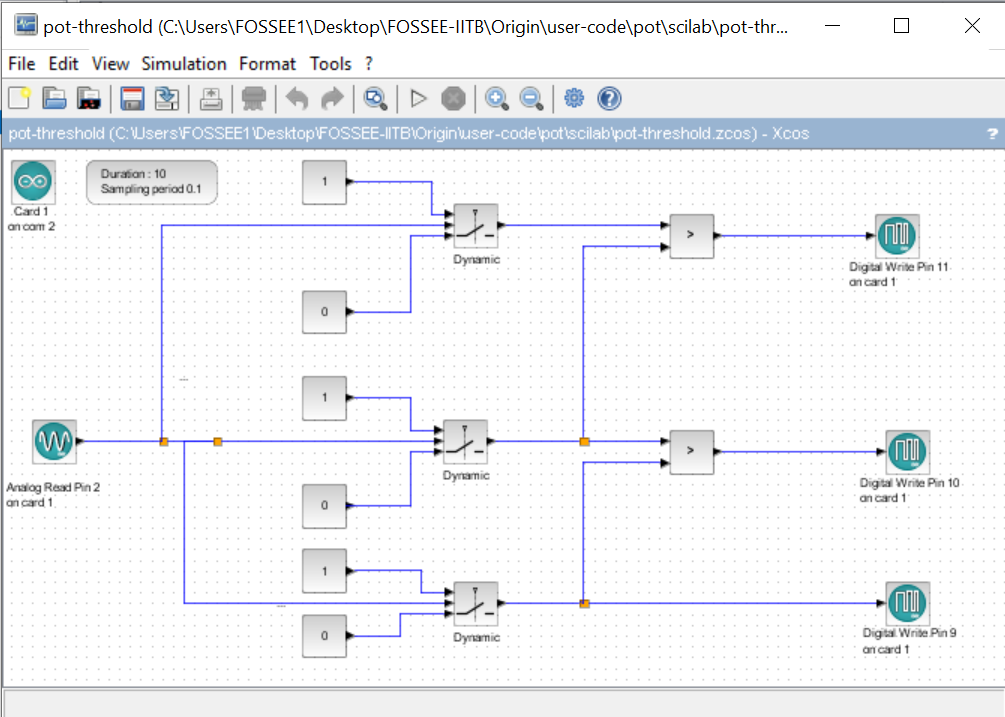
\includegraphics[width=\hgfig]{\LocPotfig/pot-threshold-1.PNG}
  \caption[Turning LEDs on through Xcos depending on the potentiometer
  threshold]{Turning LEDs on through Xcos depending on the
    potentiometer threshold.  This is what one sees when
      \LocPotscibrief{pot-threshold.zcos}, is invoked.}
  \label{fig:pot-threshold}
\end{figure}

We will next explain how to set the parameters for this simulation.
To set value on any block, one needs to right click and open the {\tt
  Block Parameters} or double click.  The values for each block is
tabulated in \tabref{tab:pot-threshold}.  All other parameters are to
be left unchanged.
  \begin{table}
    \centering
    \caption{Xcos parameters to turn on different LEDs depending on the
      potentiometer value}
    \label{tab:pot-threshold}
    \begin{tabular}{lp{2.5cm}p{2.5cm}} \hline
      Name of the block & Parameter name & Value \\ \hline
      ARDUINO\_SETUP & Identifier of Arduino Card & 1 \\
      & Serial com port number & 2\portcmd \\ \hline
      TIME\_SAMPLE & Duration of acquisition(s) & 10 \\
      & Sampling period(s) & 0.1 \\ \hline
      CONST\_m & Constant Value & 1, 0 \\ \hline
      DIGITAL\_WRITE\_SB & Digital Pin & 9(blue) \\
      & Digital Pin & 10(green) \\
      & Digital Pin & 11(red) \\ 
      & Arduino card number & 1 \\ \hline
      ANALOG\_READ\_SB & analog pin & 2 \\
      & Arduino card number & 1 \\ \hline
      SWITCH2\_m & Datatype & 1 \\
      & Pass first input & 1 \\
      & threshold & 0 \\
      & use zero crossing & 1 \\ \hline
      SWITCH2\_m & Datatype & 1 \\
      & Pass first input & 0 \\
      & threshold & 320 \\
      & use zero crossing & 1 \\ \hline
      SWITCH2\_m & Datatype & 1 \\
      & Pass first input & 0 \\
      & threshold & 900 \\
      & use zero crossing & 1 \\ \hline
      RELATIONALOP & Operator & 4 \\
      & zero crossing & 0 \\
      & Datatype & 1 \\ \hline
    \end{tabular}
  \end{table}

Note that, when the potentiometer value read by Scilab crosses either
of the thresholds, color of the LED changes. This can be observed by
rotating the knob of the potentiometer.

\begin{exercise}
List out the applications in day-to-day life where potentiometer is
being used/can be used? For example, old fan regulators used
potentiometer to change the fan speed.
\end{exercise}

